\documentclass{beamer}
\usepackage{graphicx}
\title{1.DN}
\author{Matija Leskovar, vps.št.: 23221140}
\institute{Univerza v Ljubljani, Fakulteta za Strojništvo}
\date{7. 11. 2024}

\begin{document}
\frame{\titlepage}
\begin{frame}
\frametitle{Kazalo vsebine}
\tableofcontents

\end{frame}

\begin{frame}
\frametitle{Datotkea naloga1\_1.txt}
\section{Datoteka naloga1\_1.txt}
\begin{itemize}
    \item V prvi vrstici datoteke je napisana količina, katere vrednosti so v datoteki
    \item V drugi vrstici je število preostalih vrstic po tej, le teh je 100, ter koliko podatkov je v posamezni vrstici
    \item Podatki predstavljajo čase pri katerih je bila izmerjena P(moč), vmesni razmak pa je 1/100 sekunde
    \item Uporabil sem funkcijo t=import data, ki kot argument vzame ime datoteke in v t shrani tri vrednosti, data, textdata, colheaders, najpomembnejša je vrednost data, ki vsebuje array z vrednostimi iz datoteke
\end{itemize}
\end{frame}
\begin{frame}{Graf P(t)}
\section{graf P(T)}
\begin{figure}[h]
    \centering
    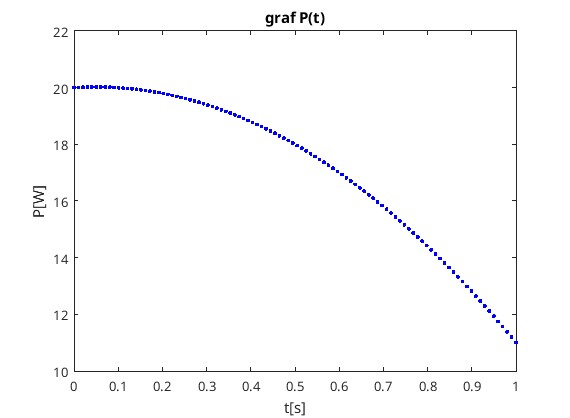
\includegraphics[width=0.5\textwidth]{P(t).jpg}
    \caption{Slika grafa P(t)}
    \label{fig:P(t)}
\end{figure}
\begin{itemize}
    \item Graf spreminjanja moči od časa. Moč pade od 20 W do 11 W v času 1 sekunde
\end{itemize}
\end{frame}
\begin{frame}{Trapezna formula in integral}
\section{Trapezna formula}
\item Formula za izračun trapezne metode:
\[
\int_{a}^{b} f(x) \, dx \approx \frac{\Delta x}{2} \left( f(x_0) + 2f(x_1) + 2f(x_2) + \dots + 2f(x_{n-1}) + f(x_n) \right)
\]
\item rešitev tega integrala po 1. formuli je:17.166496615991562
\item rešitev tega integrala po 2. formuli je:16.994831649831653
\item rešitev integrala z funkcijo trapz je:17.166496615991566
\end{frame}
\end{document}
